\documentclass[a0paper,portrait]{baposter}

\usepackage{wrapfig}
\usepackage{lmodern}
\usepackage{subfigure}
\usepackage{graphicx}
\usepackage{tikz}
\usepackage{pgfplots}
\usepackage{subcaption}
\usepackage[utf8]{inputenc} %unicode support
\usepackage[T1]{fontenc}
%\usepackage{caption}
\RequirePackage{amsmath, amssymb, amsthm, graphicx}
\usepackage{amsmath, amsthm, amssymb, latexsym}
\captionsetup[figure]{labelfont = {color = blue!20!magenta}}
\renewcommand{\figurename}{Fig.}

\selectcolormodel{cmyk}

\graphicspath{{figures/}} % Directory in which figures are stored


\newcommand{\compresslist}{%
\setlength{\itemsep}{0pt}%
\setlength{\parskip}{1pt}%
\setlength{\parsep}{0pt}%
}

\newenvironment{boenumerate}
  {\begin{enumerate}\renewcommand\labelenumi{\textbf\theenumi.}}
  {\end{enumerate}}

\begin{document}
\definecolor{darkpurple}{cmyk}{1, 0.5, 0, 0}
\definecolor{lightpurple}{cmyk}{0.7, 0.35, 0.1, 0}

\begin{poster}
{
grid=false,
headerborder=open, % Adds a border around the header of content boxes
colspacing=1em, % Column spacing
bgColorOne=white, % Background color for the gradient on the left side of the poster
bgColorTwo=white, % Background color for the gradient on the right side of the poster
borderColor=darkpurple, % Border color
headerColorOne=lightpurple, % Background color for the header in the content boxes (left side)
headerColorTwo=lightpurple, % Background color for the header in the content boxes (right side)
headerFontColor=white, % Text color for the header text in the content boxes
boxColorOne=white, % Background color of the content boxes
textborder=rounded, %rectangle, % Format of the border around content boxes, can be: none, bars, coils, triangles, rectangle, rounded, roundedsmall, roundedright or faded
eyecatcher=false, % Set to false for ignoring the left logo in the title and move the title left
headerheight=0.12\textheight, % Height of the header
headershape=rounded, % Specify the rounded corner in the content box headers, can be: rectangle, small-rounded, roundedright, roundedleft or rounded
headershade=plain,
headerfont=\Large\textsf, % Large, bold and sans serif font in the headers of content boxes
%textfont={\setlength{\parindent}{1.5em}}, % Uncomment for paragraph indentation
linewidth=2pt % Width of the border lines around content boxes
}
{}
%
%----------------------------------------------------------------------------------------
%	TITLE AND AUTHOR NAME
%----------------------------------------------------------------------------------------
%
{
\textsf %Sans Serif 
{
A proof of concept balanced mixer with the use of a digital IF power combiner to improve LO noise rejection
}
} % Poster title
{\sf\vspace{0.1em}\\
Sebastián Jorquera\textsuperscript{1}, David Monasterio\textsuperscript{1}, Franco Curotto\textsuperscript{1}, Camilo Espinoza\textsuperscript{1},
Ricardo Finger\textsuperscript{1}, Leonardo Bronfman\textsuperscript{1}
\vspace{0.1em}\\
\small{\textsuperscript{1}Departamento de Astronomía, Universidad de Chile, Camino el observatorio 1515, Santiago, Chile.
%\vspace{0.1em}\\
sebastian.jorquera@ug.uchile.cl}
}
{
\includegraphics[scale = 0.35]{logos2.png}} 

\vspace{4cm}
\headerbox{{\huge JAIN 2023}}{name = workshop, column = 0, row = 0, span = 3, boxpadding = 0.1em, cornerradius = 0.01em}{}


\headerbox{1.Balanced Mixer Architecture}{name = motivation, column = 0, below = workshop, span = 1}{
    \begin{gather*}
        I_{mixer}  = 1/2(V_{RF}+(V_{LO}+noise_{LO}))^2 + \dots
    \end{gather*}
    \begin{itemize}
        \item The quadratic term of expansion causes that the noise near the pure sinusoidal LO, got also downconverted to the IF. 
        \item This is a problem for system that uses several frequency multiplication chains to obtain a high LO frequency, since each stage adds noise to the LO.
    \end{itemize}
    
    \begin{center}
        \hspace*{1em}
        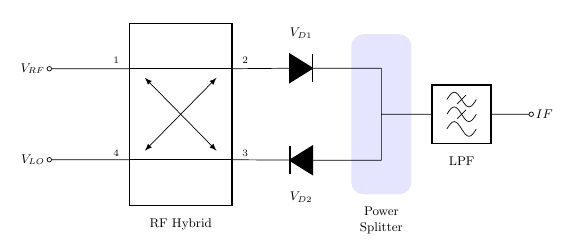
\includegraphics[width=0.9\textwidth]{images/typical_bm.png}
        \captionof{figure}{Traditional balanced mixer diagram.}
    \end{center}

    \begin{itemize} 
        \item The usage of an hybrid and two opposite orientated diodes in the balanced mixer architecture causes the cancellation of the downconverted LO noise.
        \item The non-ideal behaviour of the built components limits the LO noise cancellation.
    \end{itemize}   

}

\headerbox{2.Digitally calibrated balanced mixer}{name = antenna, column = 0, below = motivation, span = 1}{
    \begin{center}
        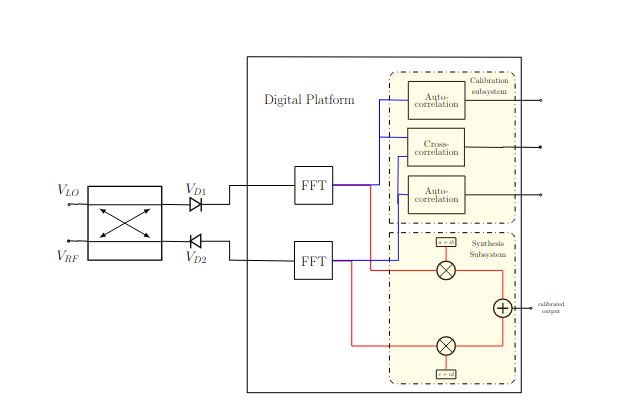
\includegraphics[width=\linewidth]{images/digital_balanced_mixer.png}
        \captionof{figure}{Digitally calibrated balanced mixer diagram.}
    \end{center}
    \begin{itemize}
        \item The proposed system consists of replacing the analog combiner with an FPGA that corrects the imbalances and combines digitally the signals.
        \item The FPGA model is composed by two subsistems.
        \begin{enumerate}
            \item Calibration subsystem: An FX correlator that measure the imabalances of the system.
            \item Synthesis subsystem: With the imbalances measured we add the correction factors previous the combination of the signals coming from the hybrid.
        \end{enumerate}
        \item Since the balanced mixer is a dual-sided band receiver, we have mapped the USB and LSB to the same IF. This is a fundamental limitation on the correction factors computation.
    \end{itemize}
}


\headerbox{3.Analog design}{name = metamaterial, span = 1, column = 1, below = workshop}{
    \begin{center}
        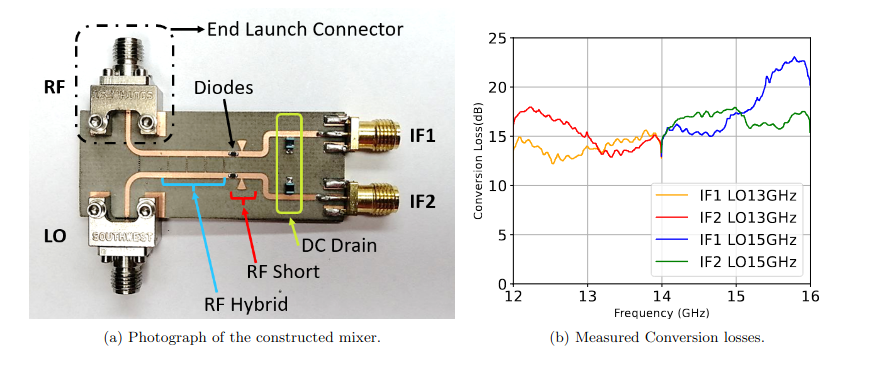
\includegraphics[width=\linewidth]{images/bm_construido.png}
        \captionof{figure}{Constructed mixer in the Ku-band.}
    \end{center}
    \begin{itemize}
        \item Since there is not commercial balanced mixer without the combiner stage, we built a mixer working in the Ku-band (13-15GHz).
        \item As the laboratory generators work injecting the minimum amount of noise, we built an artificial noise source to create a noisy LO.
        \item Since the artificial LO noise should present only in the bandwidth that its going to be downconverted we built a set of exchangeable filters. 
    \end{itemize}  
    \begin{center}
        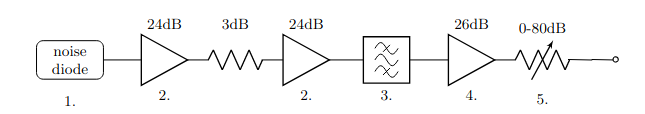
\includegraphics[width=\linewidth]{images/articial_noise_source.png}
    \end{center}
    \begin{center}
        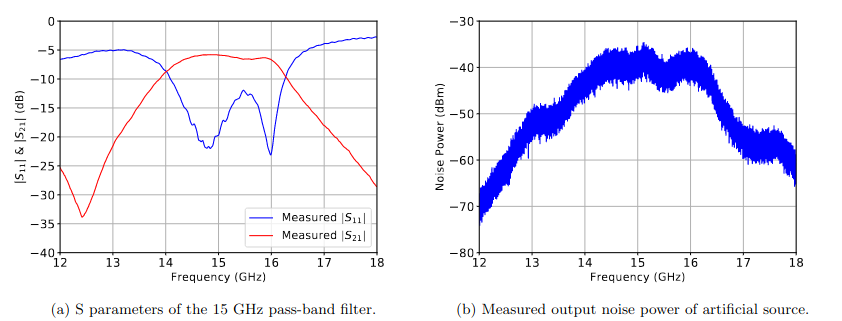
\includegraphics[width=\linewidth]{images/noise_source_meas.png}
    \end{center}
}


\headerbox{4.Test setup}{name = results, column = 1, below = metamaterial, span = 1, above=bottom}{
    \begin{center}
        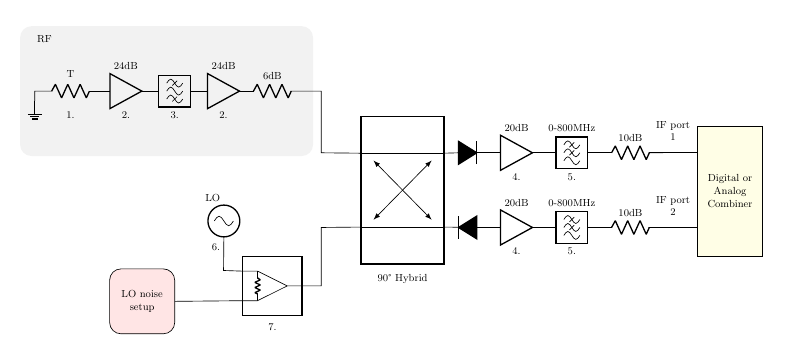
\includegraphics[width=\linewidth]{images/test_setup.png}
        \captionof{figure}{Test setup.}
    \end{center}

    \begin{itemize}
        \item As LO signal we utilized a generator combined with the artificial noise source.
        \item As RF source we utilize a noise diode to make a hot-cold test and determine the receiver temperature.
        \item To compare the performance of the proposed architecture and the standard balanced mixer, the final combiner is implemented analogically and digitally. We also measured the case of an analog combiner without added LO noise as a reference of the receiver performance.
    \end{itemize}
    
}

\headerbox{5.Results}{name = applications, column = 2, below = workshop, span = 1}{
    \begin{center}
        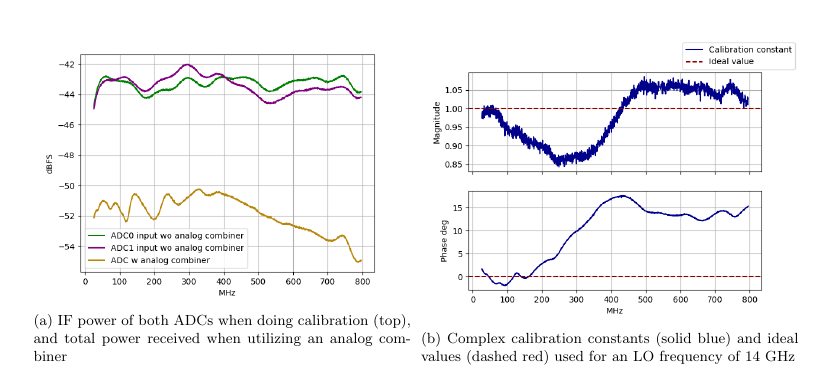
\includegraphics[width=\linewidth, height=.5\linewidth]{images/cal_meas.png}
        \captionof{figure}{Calibration measurements}
    \end{center}
    
    \begin{itemize}
        \item As the Figure 5 a) shows the amount of noise entering to the ADCs when no analog combiner is present is higher than when it is present, since when using the analog combiner the noise is rejected before the ADC. 
        \item To compute the correction factors we used the noisy LO as the test signal to characterize the system. This is done to take in account the presence of USB and LSB in the IF.
        \item The Figure 5 b) shows the complex constants calculated over the bandwidth with the LO working at 14GHz.        
    \end{itemize}

    \begin{center}
        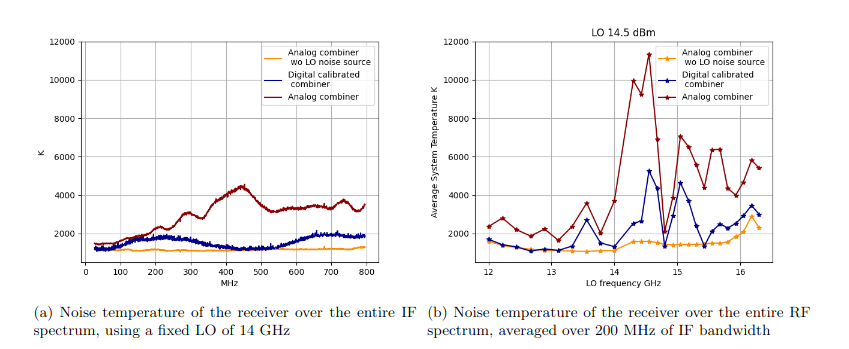
\includegraphics[width=\linewidth, height=.65\linewidth]{images/temperature.png}
        \captionof{figure}{Noise temperature measurements}
    \end{center}

    \begin{itemize}
         \item The Figure 6 a) shows the noise temperature for an LO working at 14GHz, obtaining lower temperatures than the analog combiner architecture.
         \item The Figure 6 b) shows the average noise temperature for different LO frequency values.
         \item For all LO frequencies the digitally calibrated combiner obtain lower noise temperatures than the analog combiner, and for certain points obtain comparable temperatures of the system without noise added to the LO.
    \end{itemize}
}


\headerbox{Agradecimientos}{name = greets, column = 2, below = applications, span = 1, above = bottom}{
\vspace{2em}
\begin{center}
    \large{
    Los autores agradecen el apoyo de ANID a través de sus fondos Basal ACE210002, FONDECYT 1221662 y FONDEF ID21-10359
    }
\end{center}

}

\end{poster}

\end{document}
